\documentclass{article}

\usepackage[italian]{babel}
\usepackage[utf8]{inputenc}
\usepackage[export]{adjustbox}
\usepackage{wrapfig}
\usepackage{graphicx}
\usepackage{float}
\usepackage{hyperref}
\usepackage{natbib}
\usepackage[margin=2.5cm]{geometry}
\usepackage{minted}
\usepackage{graphicx}
\usepackage{subcaption}
\usepackage{listings}
\usepackage{color}

\definecolor{pblue}{rgb}{0.13,0.13,1}
\definecolor{pgreen}{rgb}{0,0.5,0}
\definecolor{pred}{rgb}{0.9,0,0}
\definecolor{pgrey}{rgb}{0.46,0.45,0.48}
\lstset{language=Java,
  showspaces=false,
  showtabs=false,
  breaklines=true,
  showstringspaces=false,
  breakatwhitespace=true,
  commentstyle=\color{pgreen},
  keywordstyle=\color{pblue},
  stringstyle=\color{pred},
  basicstyle=\ttfamily
}

\title{ATTSW Exam: Gradle come sostituto di Maven}
\author{Gabriele Puliti - \texttt{5300140} - \href{mailto:gabriele.puliti@stud.unifi.it}{\textit{gabriele.puliti@stud.unifi.it}}}
\date{Marzo 2018}

\begin{document}

\pagenumbering{Roman}
\maketitle

\newpage
\tableofcontents
\newpage

\begin{flushleft}

\pagenumbering{Roman}

\section{Introduzione: Gradle} % https://github.com/gradle/gradle 
Gradle è un progetto open source che fornisce un tool di build automation, che può essere un ottimo sostituto di Maven. Offre un modello in grado di sostenere l'intero ciclo di vita dello sviluppo del software ed è stato progettato per supportare build automation attraverso più linguaggi e piattaforme. Nel nostro caso considereremo questo tool per lo sviluppo di software Java.

\subsection{Differenze tra Gradle e Maven} % https://gradle.org/maven-vs-gradle/
Ci sono molte differenze tra questi due tools: flessibilità, performance, gestione delle dipendenze e molto altro. La configurazione di Gradle in un progetto ha una convenzione molto più facile e comprensibile rispetto alla tediosa e a volte impossibile configurazione del pom.xml di Maven, anche se entrambi usano dei metodi di miglioramento della velocità di esecuzione delle build. Grandle usufruisce di:
\begin{itemize}
    \item \textbf{Incrementality:} evitando il lavoro di monitoraggio dei task di I/O eseguendo solo il necessario e quando possibile processare solo i files che sono cambiati;
    \item \textbf{Build Cache:} utilizza un sistema di cache riusando gli outputs di altre build Gradle con gli stessi inputs;
    \item \textbf{Deamon:} sfrutta un long-lived process che mantiene tutte le informazioni in memoria.
\end{itemize}
Queste 3 caratteristiche rendono Gradle molto veloce, ad esempio una build Gradle con Maven verrebbe completata con un tempo 3 volte maggiore. Tutto questo è anche possibile grazie a un sistema di esecuzioni parallele di task e intra-task.
\begin{figure}[H]
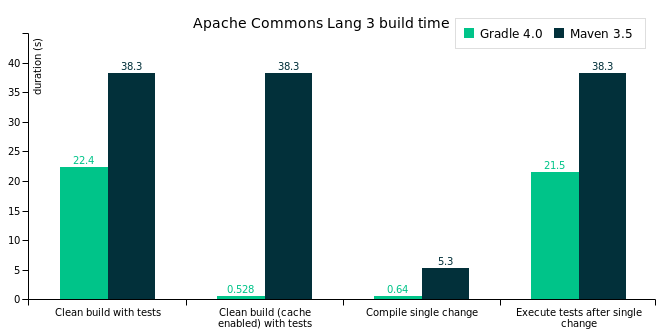
\includegraphics[scale=0.70]{introduction/performance.png}
\end{figure} 
% https://docs.gradle.org/current/userguide/userguide.html

\subsection{Installazione}
L'istallazione di Gradle può essere fatta in più modi: tramite installazione manuale o utilizzando un package manager (tutte le informazioni possono essere trovate in \textbf{\href{https://gradle.org/install/}{questo link}}). Personalmente consiglio l'utilizzo del software development kit manager \textbf{\href{http://sdkman.io/}{SDKMAN!}} che non solo permette l'installazione molto facilitata di Gradle, ma anche della JVM e di tanti altri tools.

\subsubsection{installazione tramite SDKMAN!}
L'installazione si basa su 2 semplici comandi:
\begin{verbatim}
  $ curl -s "https://get.sdkman.io" | bash
  
  $ source "$HOME/.sdkman/bin/sdkman-init.sh" \end{verbatim}
A questo punto se tutto è andato a buon fine SDKMAN! è stato installato correttamente, è possibile verificarlo digitando il comando su terminale:
\begin{verbatim}
  $ sdk version \end{verbatim}
l'output risultante dovrebbe essere qualcosa del tipo:
\begin{verbatim}
  SDKMAN 5.5.15+284 \end{verbatim}
Ora è possibile procedere con l'installazione di Gradle. Prima di tutto visualizziamo la lista delle versioni di Gradle:
\begin{verbatim}
  $ sdk list gradle \end{verbatim}
L'output corrispondente sarà:
\begin{verbatim}
================================================================================
Available Gradle Versions
================================================================================
     4.4.1                4.2-rc-2             3.0                  2.10           
     4.4-rc-6             4.2-rc-1             2.9                  2.1            
     4.4-rc-5             4.2                  2.8                  2.0            
     4.4-rc-4             4.1                  2.7                  1.9            
     4.4-rc-3             4.0.2                2.6                  1.8            
     4.4-rc-2             4.0.1                2.5                  1.7            
     4.4-rc-1             4.0                  2.4                  1.6            
     4.4                  3.5.1                2.3                  1.5            
     4.3.1                3.5                  2.2.1                1.4            
     4.3-rc-4             3.4.1                2.2                  1.3            
     4.3-rc-3             3.4                  2.14.1               1.2            
     4.3-rc-2             3.3                  2.14                 1.12           
     4.3-rc-1             3.2.1                2.13                 1.11           
     4.3                  3.2                  2.12                 1.10           
     4.2.1                3.1                  2.11                 1.1            
================================================================================
+ - local version
* - installed
> - currently in use
================================================================================ \end{verbatim}
La versione che vogliamo installare è quella più recente che in questo caso è la 4.4.1, possiamo quindi eseguire il comando:
\begin{verbatim}
  $ sdk install gradle 4.4.1 \end{verbatim}
appena il download e l'installazione sarà finita possiamo verificare il completamento tramite:
\begin{verbatim}
  $ gradle -v \end{verbatim}
che non solo stamperà su terminale la versione di Gradle, ma anche:
\begin{itemize}
  \item \href{http://www.groovy-lang.org/}{Groovy} (linguaggio di programmazione usato per scrivere i file di configurazione)
  \item Ant (software usato per le build delle Java applications)
  \item Java Virtual Machine
  \item sistema operativo in uso
\end{itemize}
se l'output ha queste informazioni allora Gradle è stato completamente installato. SDKMAN! si preoccupa anche di creare la variabile \$GRADLE\_HOME che è possibile visualizzare con il comando 
\begin{verbatim} 
    $ echo $GRADLE_HOME \end{verbatim} 
Se ci sono errori di tipo Java, i problemi possono essere:
\begin{itemize}
  \item Gradle non riesce a trovare la jdk, problema risolvibile installando java con sdkman con il comando 
  \begin{verbatim}
    $ sdk install java <versione>  \end{verbatim}
  \item Java è aggiornato alla versione 9 o superiori (infatti attualmente Gradle 4.4.1 non è aggiornato per versioni superiori alla 8), basterà fare un downgrade ad una versione precedente (possibile farlo anche tramite SDKMAN!).
\end{itemize}
In entrambi i casi sarà necessario anche comunicare al sistema la versione da usare: 
\begin{verbatim}  
    $ sdk dafault java <versione_installata> \end{verbatim} 
per essere sicuri che è stata installata la giusta versione di java possiamo controllare gli outputs dei seguenti comandi:
\begin{itemize}
  \item \begin{verbatim} $ echo $JAVA_HOME \end{verbatim}
  \item \begin{verbatim} $ java -version \end{verbatim}
\end{itemize}
il primo comando dovrà restituire in output il giusto percorso della JVM installata, il secondo serve a controllare la versione java attualmente in uso.


\newpage

\pagenumbering{arabic}
\subsection{Tasks \& Task Dependencies}
Come in Maven ci sono i goals, in Gradle ci sono i tasks ognuno dei quali ha il suo scopo definito nella sua implementazione. L'implementazione dei tasks viene fatta in un file di configurazione solitamente nominato build.gradle. Creaiamo quindi una cartella source in cui inserire la nostra configurazione di gradle e creiamo il file build.gradle in cui andremo a inserire:

\begin{verbatim}
    description = 'Example of Task'

    task dependenceZero {
        description = 'Build Dependence Zero'
        doFirst {
            println 'First Zero'
        }
        doLast {
            println 'Last Zero'
        }
    }

    task dependenceOne(dependsOn: [dependenceZero]) {
        description = 'Build Dependence One'
        doFirst {
            println 'First One'
        }
        doLast {
            println 'Last One'
        }
    }

    task dependenceTwo {
        description = 'Build Dependence Two'
        doFirst {
            println 'First Two'
        }
        doLast {
            println 'Last Two'
        }
    }

    task mainTask(dependsOn: [dependenceOne, dependenceTwo]) {
        description = 'Build Main Task'
        doFirst {
            println 'First MainTask'
        }
        doLast {
            println 'Last MainTask'
        }
    }
\end{verbatim}

In questa build abbiamo definito 4 task: dependenceZero, dependeceOne, dependenceTwo e mainTask. Nella definizione del task può essere usata la parola \textsc{dependsOn} per indicare che il task definito dipende da uno o più task. Nel caso di dependenceOne abbiamo una sola dipendenza che è dependenceZero, nel caso invece di taskMain si hanno 2 dipendenze che sono dependenceOne e dependenceTwo. Possiamo notare che si è data una descrizione sia dei tasks che della build, questo non serve nella pratica ma è buona norma dare sempre una spiegazione sia della build che dei nuovi task che si creano. All'interno dei tasks si nota che ci sono definite delle azioni: doFirst e doLast, quando sarà eseguita la build di un task verrà eseguita prima doFirst e infine doLast. Con la configurazione precedente abbiamo creato un albero delle dipendenze di questo tipo:

\begin{figure}[H]
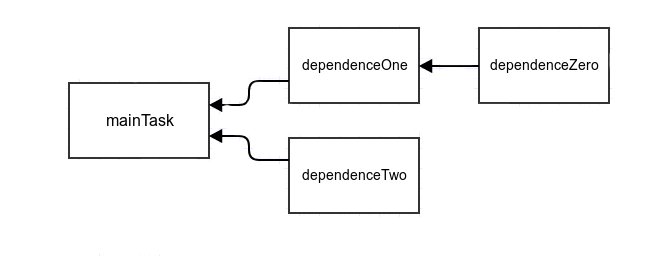
\includegraphics[scale=0.40]{HowToUse/1Task/task_taskDep/graphDep.png}
\end{figure}

Le builds di gradle vengono eseguite usando il comando da terminale \texttt{\$ gradle taskName}, per l'esempio è possibile quindi eseguire le builds:
\begin{itemize}
    \item \begin{verbatim} $ gradle dependenceZero \end{verbatim}
    \item \begin{verbatim} $ gradle dependenceOne \end{verbatim}
    \item \begin{verbatim} $ gradle dependenceTwo \end{verbatim}
    \item \begin{verbatim} $ gradle mainTask \end{verbatim}
\end{itemize}
Ma è anche possibile eseguire più task contemporaneamente, per esempio:
\begin{itemize}
    \item \begin{verbatim} $ gradle dependenceZero mainTask\end{verbatim}
    \item \begin{verbatim} $ gradle dependenceOne dependenceTwo \end{verbatim}
    \item \begin{verbatim} $ gradle dependenceOne dependenceTwo mainTask\end{verbatim}
\end{itemize}
Considerando che il mainTask è dipendente da dependenceOne e dependenceTwo, l'ultimo esempio non aggiunge niente di più alla build dato che verrebbero comunque eseguiti i 2 tasks. Se eseguiamo infatti \begin{verbatim}$ gradle mainTask \end{verbatim} e poi \begin{verbatim}$ gradle dependenceOne dependenceTwo mainTask\end{verbatim} otterremo il solito output, che è il seguende:
\label{outMainTask}
\begin{verbatim}
> Task :dependenceZero 
First Zero
Last Zero

> Task :dependenceOne 
First One
Last One

> Task :dependenceTwo 
First Two
Last Two

> Task :mainTask 
First MainTask
Last MainTask


BUILD SUCCESSFUL in 0s
4 actionable tasks: 4 executed\end{verbatim} 


\subsection{Approfondimenti}
Andiamo ad approfondire le azioni che è possibile fare tramite il terminale.
\subsubsection{Abbreviazione dei nomi}
È possibile abbreviare il nome del task da eseguire stando però attenti ad identificarlo unicamente, per esempio se volessi eseguire il task \textbf{dependenceTwo} potrei farlo semplicemente con il comando:
\begin{verbatim}
    $ gradle depTw \end{verbatim}
considerando i task creati precedentemente notiamo che il task è univocamente identificato.

\subsubsection{Escludere i task}
È possibile escludere un task di una build, aggiungendo come argomento il task da escludere preceduto da -x:
\begin{verbatim}
    $ gradle <task_da_eseguire> -x <task_da_escludere> \end{verbatim}
questo viene usato al fine di eliminare un task inutile per lo scopo della build che abbiamo intenzione di eseguire. Riprendendo l'output di \begin{verbatim}   $ gradle mainTask \end{verbatim} notiamo che vengono eseguiti tutti i tasks definiti nella build.gradle (a pagina \pageref{outMainTask}), se volessimo escludere dependenceOne dalla build allora dovremo eseguire:
\begin{verbatim}
    $ gradle mainTask -x dependenceOne \end{verbatim}
Otteniamo in questo modo in output:
\begin{verbatim}
> Task :dependenceTwo 
First Two
Last Two

> Task :mainTask 
First MainTask
Last MainTask


BUILD SUCCESSFUL in 0s
2 actionable tasks: 2 executed
\end{verbatim}
Possiamo notare che non verrà eseguito nemmeno il task dependenceZero perchè è una dipendenza del task dependenceOne.

\subsubsection{Selezionare la build da eseguire}
Consideriamo che esista in una subdirectory chiamata subdir una build chiamata subbild.gradle, partendo dalla directory source è possibile eseguire questa build eseguendo il comando:
\begin{verbatim}
    $ gradle -b subdir/subbuild.gradle <task_da_eseguire> \end{verbatim}
Questa particolare funzione serve soprattutto ai progetti multi-builds, in cui è necessario avere a disposizione più di una build di riferimento.

\subsubsection{Forzare l'esecuzione di un task} 
A causa della Gradle cache è possibile che un task o più di uno non vengano eseguiti perchè marcati come UP-TO-DATE (anche se dalla versione Gradle 4.0 non viene più mostrato in output), in questo caso è possibile forzarne l'esecuzione con:
\begin{verbatim}
    $ gradle --rerun-tasks <tasks_da_eseguire> \end{verbatim}
    
\subsubsection{Continuare la build quando si verifica un errore}
Se durante una build un task fallisce, Gradle di default interromperà l'esecuzione e farà fallire anche la build. Questo permette alla build di completare velocemente, ma il fallimento anticipato della build potrebbe nascondere altri problemi che possono presentarsi in altri tasks. A volte è quindi necessario imporre ad una build di gradle di continuare nonostante il fallimento di uno o più tasks, questo è possibile usando l'opzione \texttt{--continue}:
\begin{verbatim}
    $ gradle <tasks_da_eseguire> --continue\end{verbatim}
In questo modo verranno eseguiti tutti i tasks e solo al completamento della build saranno resi noti gli errori.

\subsubsection{Ottenere informazioni generali} 
Per visualizzare una lista dei principali tasks eseguibili è possibile eseguire il task \begin{verbatim}    $ gradle tasks\end{verbatim} l'output di questa build sarà:
\begin{verbatim}
> Task :tasks 

------------------------------------------------------------
All tasks runnable from root project - Example of Task
------------------------------------------------------------

Build Setup tasks
-----------------
init - Initializes a new Gradle build.
wrapper - Generates Gradle wrapper files.

Help tasks
----------
buildEnvironment - Displays all buildscript dependencies declared in root project 'src'.
components - Displays the components produced by root project 'src'. [incubating]
dependencies - Displays all dependencies declared in root project 'src'.
dependencyInsight - Displays the insight into a specific dependency in root project 'src'.
dependentComponents - Displays the dependent components of components in root project 'src'. 
[incubating]
help - Displays a help message.
model - Displays the configuration model of root project 'src'. [incubating]
projects - Displays the sub-projects of root project 'src'.
properties - Displays the properties of root project 'src'.
tasks - Displays the tasks runnable from root project 'src'.

To see all tasks and more detail, run gradle tasks --all

To see more detail about a task, run gradle help --task <task>


BUILD SUCCESSFUL in 0s
1 actionable task: 1 executed
\end{verbatim}

come dice l'output, per visualizzare la lista di tutti i tasks eseguibili nel nostro project è necessario eseguire la build del task \begin{verbatim}$ gradle tasks --all \end{verbatim} noteremo che in questo caso verranno visualizzati anche i tasks che abbiamo precedentemente creato (dependenceZero, dependenceOne, dependenceTwo, mainTask con le relative descrizioni):
\begin{verbatim}
> Task :tasks 

------------------------------------------------------------
All tasks runnable from root project - Example of Task
------------------------------------------------------------

Build Setup tasks
-----------------
init - Initializes a new Gradle build.
wrapper - Generates Gradle wrapper files.

Help tasks
----------
buildEnvironment - Displays all buildscript dependencies declared in root project 'src'.
components - Displays the components produced by root project 'src'. [incubating]
dependencies - Displays all dependencies declared in root project 'src'.
dependencyInsight - Displays the insight into a specific dependency in root project 'src'.
dependentComponents - Displays the dependent components of components in root project 'src'. 
[incubating]
help - Displays a help message.
model - Displays the configuration model of root project 'src'. [incubating]
projects - Displays the sub-projects of root project 'src'.
properties - Displays the properties of root project 'src'.
tasks - Displays the tasks runnable from root project 'src'.

Other tasks
-----------
dependenceOne - Build Dependence One
dependenceTwo - Build Dependence Two
dependenceZero - Build Dependence Zero
mainTask - Build Main Task


BUILD SUCCESSFUL in 0s
1 actionable task: 1 executed
\end{verbatim}
Se invece vogliamo informazioni più specifiche riguardo un singolo task la build da fare è 
\begin{verbatim}
    $ gradle help --task <nome_del_task>\end{verbatim}
per esempio eseguiamo:
\begin{verbatim}
    $ gradle help --task mainTask\end{verbatim}
otterremo una descrizione specifica del task mainTask:
\begin{verbatim}
> Task :help 
Detailed task information for mainTask

Path
     :mainTask

Type
     Task (org.gradle.api.Task)

Description
     Build Main Task

Group
     -\end{verbatim}

\subsubsection{Build scan}
Una funzione molto interessante di Gradle è la possibilità di poter pubblicare la propria build, questo permette di avere un report completo e condivisibile. Per utilizzare questa funzionalità è necessario aggiungere alla build di un task l'opzione \texttt{--scan}:
\begin{verbatim}    $ gradle <task_da_eseguire> --scan \end{verbatim}
Al completamento della build del task verrà richiesto di accettare i termini di uso di questo servizio. Una volta accettati verrà fornito un link alla build pubblicata in cui sarà richiesta una mail di riferimento per confermare la pubblicazione della build. Prendendo come esempio eseguiamo il comando:
\begin{verbatim}
    $ gradle mainTask --scan\end{verbatim}
l'output risultante sarà:
\begin{verbatim}
> Task :dependenceZero 
First Zero
Last Zero

> Task :dependenceOne 
First One
Last One

> Task :dependenceTwo 
First Two
Last Two

> Task :mainTask 
First MainTask
Last MainTask


BUILD SUCCESSFUL in 1s
4 actionable tasks: 4 executed

Publishing a build scan to scans.gradle.com requires accepting the Gradle Terms of Service 
defined at https://gradle.com/terms-of-service. Do you accept these terms? [yes, no] 
yes
Gradle Terms of Service accepted.

Publishing build scan...
https://scans.gradle.com/s/qcc4vkuegibig
\end{verbatim}
cliccando sul sito e seguendo le indicazioni, il risultato finale sarà:
\begin{figure}[H]
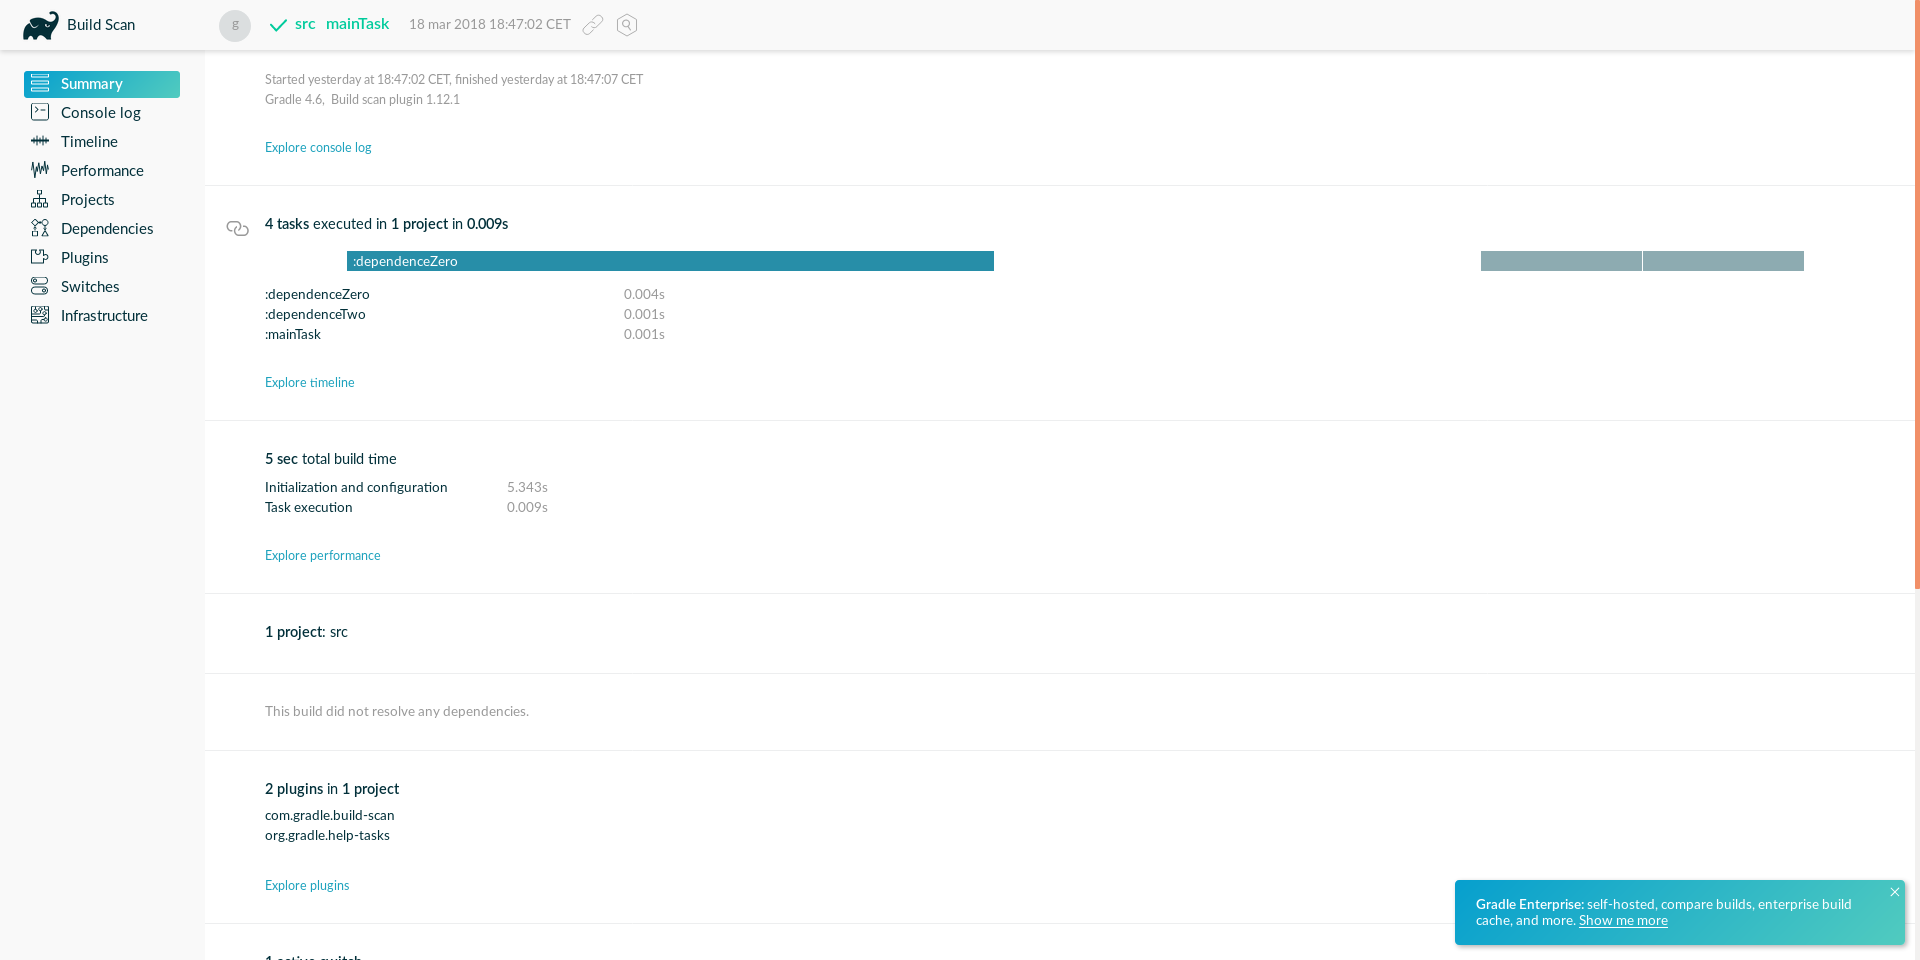
\includegraphics[scale=0.25]{HowToUse/1Task/insights/gradleScan.png}
\end{figure}
\newpage
\section{Project, Wrapper \& Deamon}
Potete trovare un tutorial guidato a questo link: \href{https://github.com/Wabri/ATTSW_Exam/tree/master/gradle.example/second}{\textsc{github.com/Wabri/ATTSW\_Exam/tree/master/gradle.example/second}}

\subsection{Creazione di un nuovo progetto Gradle}
Creare un progetto Gradle è molto semplice sfruttando direttamente il task di default \textsc{init}. Creiamo una cartella in cui eseguiremo da terminale il comando:
\begin{verbatim}
    $ gradle init\end{verbatim}
Notiamo che nella directory sono stati creati 4 file e 1 cartella:
\begin{itemize}
    \item \texttt{build.gradle} e \texttt{settings.gradle}: sono i file di configurazione
    \item \texttt{gradlew}, \texttt{gradlew.bat} e la directory \texttt{gradle}: sono i file corrispondenti al wrapper
\end{itemize}
Abbiamo già trattato il file di configurazione build.gradle (pagina \pageref{buildGradle}). Il file settings.gradle è anch'esso uno script Groovy dove vengono indicati quali progetti parteciperanno alla build. Questo task crea un progetto di default, ma è possibile essere più specifici in quanto il task \textsc{init} con l'opzione \texttt{--type} può assumere come argomento una tipologia di progetto. Assumiamo che il progetto che vogliamo creare sia una applicazione java, il comando da eseguire sarà:
\begin{verbatim}
    $ gradle init --type java-application\end{verbatim}
Rispetto al comando precedente verrà creata una directory \texttt{src} in più che sarà specifica per il linguaggio java:
\begin{itemize}
    \item \texttt{main/java/App.java}: che è un file preimpostato il cui contenutò sarà un semplice main che stamperà il consueto \textsc{Hello World!}
    \item \texttt{test/java/AppTest.java}: in cui viene testato il metodo contenuto nella classe App.java
\end{itemize}
Spieghiamo a questo punto i file del wrapper precedentemente indicati.


\subsection{Wrapper}
Molto spesso prima di poter usufruire di uno strumento di sviluppo è necessaria una installazione. Gradle mette a disposizione uno script che permette di usare tutte le sue funzionalità evitando di installare Gradle su tutte le macchine di sviluppo, questo strumento viene chiamato Gradle Wrapper. Se in un progetto è stato settato il Wrapper è possibile eseguire le builds sostituendo il comando \texttt{gradle} con il comando \texttt{./gradlew} (se si lavora con sistema operativo windows il comando è \texttt{./gradlew.bat}). Se più persone lavorano a un progetto può capitare che ci siano differenze tra le versioni di uno strumento, nel caso del wrapper non è possibile sbagliare perchè la sua versione è insita durante la sua creazione o durante il suo upgrade (o downgrade). Quindi è sempre consigliato l'uso del wrapper e lasciare tutte le sue informazioni anche nella repository del VCS usato. Per creare il wrapper in un progetto è necessario eseguire il comando:
\begin{verbatim}
    $ gradle wrapper\end{verbatim}
Il comando creerà 4 files:
\begin{itemize}
    \item \textbf{gradlew}: script shell per eseguire il wrapper in sistemi Unix
    \item \textbf{gradlew.bat}: file batch per eseguire il wrapper in sistemi Windows
    \item \textbf{gradle/wrapper/gradle-wrapper.properties}: file di configurazione delle proprietà del Wrapper
    \item \textbf{gradle/wrapper/gradle-wrapper.jar}: contiene il codice effettivo per eseguire le build Gradle
\end{itemize}
Questi sono i file di cui ha bisogno il wrapper per poter essere usato. Ovviamente Quando il wrapper viene creato la sua versione sarà quella di Gradle attualmente installato sulla macchina, è possibile specificare in vari modi quale versione usare:
\begin{enumerate}
    \item eseguire il solito comando con l'aggiunta dell'argomento \texttt{--gradle-version} con il numero della versione:
\begin{verbatim}
    $ gradle wrapper --gradle-version <numero_versione> \end{verbatim}
oppure se già inserito il wrapper:
\begin{verbatim}
    $ ./gradlew wrapper --gradle-version <numero_versione> \end{verbatim}
per esempio se volessimo passare dalla versione attuale alla versione 2.0 basterà eseguire il comando:
\begin{verbatim}
    $ ./gradlew wrapper --gradle-version 2.0 \end{verbatim}
dopo aver eseguito il download della versione, l'output corrispondente sarà:
\begin{verbatim}
------------------------------------------------------------
Gradle 2.0
------------------------------------------------------------
Build time:   2014-07-01 07:45:34 UTC
Build number: none
Revision:     b6ead6fa452dfdadec484059191eb641d817226c
Groovy:       2.3.3
Ant:          Apache Ant(TM) version 1.9.3 compiled on December 23 2013
JVM:          1.8.0_161 (Oracle Corporation 25.161-b12)
OS:           Linux 4.13.0-37-generic amd64
\end{verbatim}
(il task wrapper non esisteva fino alla versione 3.0, eseguire quindi questo task con versioni precedenti risulterebbe in un fallimento della build).
    \item modificare direttamente il file gradle-wrapper.properties in cui ci sarà:
\begin{verbatim}
    distributionUrl=https\://services.gradle.org/distributions/gradle-4.4.1-bin.zip \end{verbatim}
    che è il tipo di distribuzione usata attualmente dal wrapper. Per passare alla versione 2.0 possiamo modificare questa riga con:
\begin{verbatim}
    distributionUrl=https\://services.gradle.org/distributions/gradle-2.0-bin.zip \end{verbatim}
    eseguendo poi un qualsiasi comando la versione sarà aggiornata.
    \item infine è possibile specificarlo direttamente modificando il file build.gradle aggiungendo un task chiamato wrapper che estenderà la classe Wrapper:
\begin{verbatim}
    task wrapper(type: Wrapper) {
        gradleVersion = '2.0'
    } \end{verbatim}
    in questo modo viene effettivamente fatto un override del task wrapper. A questo punto per aggiornare alla versione indicata basterà eseguire il comando:
\begin{verbatim}
    $ ./gradlew wrapper \end{verbatim}
    
\end{enumerate}
In ogni caso possiamo visualizzare la versione usata dal wrapper con il comando:
\begin{verbatim}
    $ ./gradlew --version \end{verbatim}
Il wrapper è altamente configurabile sia come proprietà sia come versionamento. Per esempio riprendendo il punto 3 della lista precedente, se non si vuole specificare tutte le volte il tipo di distribuzione voluta è possibile inserire un altro campo all’interno del task wrapper \texttt{distributionType} a cui assegneremo \texttt{Wrapper.DistributionType.ALL}:
\begin{lstlisting}[frame=single]
task wrapper(type: Wrapper) {
    gradleVersion = '4.6'
    distributionType = Wrapper.DistributionType.ALL
}
\end{lstlisting}
In questo modo verrà scaricata tutta la distribuzione e non solo i file binari.

\subsection{Deamon}
Gradle viene eseguito sulla Java virtual machine (JVM) e usa librerie di supporto che necessitano una inizializzazione, entrambi allungano il processo di esecuzione iniziale della build allungando i tempi di attesa. Questo problema viene risolto usando un Deamon che mantiene le informazioni della build in background velocizzando le esecuzioni successive alla prima, mantenendo le informazioni in memoria pronte all'uso. Una build di gradle è possibile eseguirla con o senza il deamon, indicando nelle proprietà di Gradle quando usarlo e se usarlo. Il daemon permette non solo di evitare l'avviamento della JVM, ma ha anche un sistema di cache in cui sono immagazzinati: struttura del progetto, files, tasks e molto altro. Ovviamente se il progetto viene eseguito in contenitori temporanei, tipo un server di continuous integration (CI), è sconsigliato l'uso del deamon in quanto questi non riutilizzano lo stesso processo ma ne creano uno nuovo, quindi l'uso del deamon non solo è inutile ma ridurrà anche le prestazioni dato che dovrà rieseguire il deamon di gradle e ricreare la cache. Per controllare i processi deamon attivi sulla macchina basterà eseguire il comando:
\begin{verbatim}
    $ gradle --status \end{verbatim}
che restituirà il pid, lo stato e la versione di gradle usata dal deamon. Ad esempio se abbiamo un progetto in cui è usata la versione di gradle 3.0 avremo un risultato di questo tipo:
\begin{verbatim}
    PID STATUS   INFO
  16463 IDLE     3.0 \end{verbatim}


\subsection{Tutorial}
Il tutorial di seguito è possibile anche trovarlo al link: \href{https://github.com/Wabri/ATTSW_Exam/blob/master/gradle.example/first/}{\texttt{github.com/Wabri/ATTSW\_Exam/blob/master/gradle.example/second/}}.
\begin{enumerate}
    \item Creare una cartella gradle.example/second
    \item Eseguire la build:
\begin{verbatim}
    $ gradle init --type java-application
\end{verbatim}
    \item Usare il wrapper per controllare la versione attualmente in uso dal progetto:
\begin{verbatim}
    ./gradlew --version\end{verbatim}
    \item Cambiare la versione del wrapper alla 2.0:
\begin{verbatim}
    $ ./gradlew wrapper --gradle-version 2.0\end{verbatim}
    \item Controllare se la versione del wrapper è stata cambiata:
\begin{verbatim}
    $ ./gradlew --version\end{verbatim}
    \item Fare l'upgrade alla 3.0 del wrapper usando le properties, modificando il campo \texttt{distribuitionUrl}:
\begin{verbatim}
distributionUrl=https\://services.gradle.org/distributions/gradle-3.0-bin.zip \end{verbatim}
    \item Controllare se la versione del wrapper è stata cambiata
    \item Modificare il build.gradle per impostare la versione del wrapper alla 4.6:
\begin{lstlisting}[frame=single]
task wrapper(type: Wrapper) {
    gradleVersion = '4.6'
}
\end{lstlisting}
    \item La versione non sarà modificata fintanto che non sarà eseguito il task \texttt{wrapper}, eseguire quindi la build:
\begin{verbatim}
    $ ./gradlew wrapper\end{verbatim}
    \item Controllare se la versione del wrapper è stata cambiata
    \item Impostare All come tipo di distribuzione da usare per il wrapper, aggiungere quindi il campo \texttt{distributionType}:
\begin{lstlisting}[frame=single]
task  wrapper(type: Wrapper) {
    gradleVersion ='4.6'
    distributionType = Wrapper.DistributionType.ALL
}
\end{lstlisting}
    \item Eseguire la build del task \texttt{wrapper} per aggiornare la distribuzione usata dal wrapper
    \item Visualizzare lo stato attuale dei daemon attualmente in esecuzione:
\begin{verbatim}
    $ ./gradlew --status\end{verbatim}
    \item Eseguire il task \texttt{test} usando il daemon:
\begin{verbatim}
    $ ./gradlew --daemon test\end{verbatim}
    (Notare che se viene rieseguita questa build il tempo di esecuzione risulta essere nullo)
    \item Eseguire lo stesso task precedente senza usare il daemon:
\begin{verbatim}
    $ ./gradlew --no-daemon test\end{verbatim}
    (Notare che non usando il daemon il tempo di esecuzione non sarà nullo)
    \item Stoppare il daemon attivo attualmente usato:
\begin{verbatim}
    $ ./gradlew --stop <PID>\end{verbatim}
\end{enumerate}
\newpage
\section{Dependency Management}
Una delle parti più importanti di uno strumento di questo tipo è la gestione delle dipendenze che si divide in 2 parti: incoming files e outgoing files. Gradle ha bisogno di conoscere di cosa il nostro progetto ha bisogno per poter essere compilato ed eseguito le così dette dipendenze (dipendencies) che in questo caso sono gli incoming files. Gli outgoing files sono invece tutto ciò che il progetto produce, definite pubblicazioni (pubblications). Le dipendenze vengono specificate in forma di modules, è quindi necessario indicare dove si trovano questi modules in modo tale che Gradle li possa scaricare e impostare per il progetto che stiamo sviluppando. La posizione dove è possibile trovare i modules è definita repository, è necessario quindi dichiarare le repositories usate per le dipendenze volute. Ci sono 2 tipi di repository: 
\begin{enumerate}
    \item esterne, in questo caso la repository si trova in un server online adibito alla raccolta di modules
    \item interne, la repository è una cartella locale al progetto
\end{enumerate}
Per quanto riguarda quelle esterne Gradle si occuperà di scaricarle. E' possibile che alcune dipendenze vengano usate in più progetti, gradle mantiene quindi una cache locale, chiamata dependency cache, in cui salverà i modules già scaricati in modo da evitare di effettuare il download ad ogni build. Possiamo quindi immaginare che il ciclo di risoluzione delle dipendenze esterne sarà questo:
\begin{enumerate}
    \item ricerca delle dipendenze esterne nella cache locale
    \item se non si trovano nella cache locale si controlla se esistono nelle repository specificate
    \item se sono state trovate, vengono scaricate e inserite nella cache locale
\end{enumerate}
Nell'immagine è possibile vedere il percorso specifico che effettua la dependency resolution di Gradle:
\begin{figure}[H]
\centering
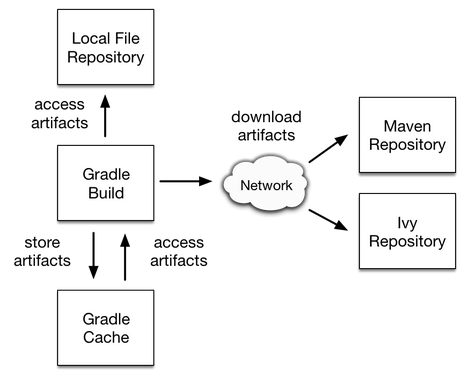
\includegraphics[width=0.4\linewidth]{HowToUse/3DependencyManagement/depMan.png}
\end{figure}
Analizziamo ora il caso di un progetto java.

\subsection{Dichiarazione delle dipendenze}
Prima di tutto è necessario indicare in che linguaggio il nostro progetto viene rilasciato (consideriamo d'ora in poi solo il caso di Java), per farlo aggiungiamo in testa al file build.gradle:
\begin{verbatim}
apply plugin: 'java' \end{verbatim}
A questo punto per poter usufruire di una dipendenza è necessario specificare da dove Gradle deve andare a prenderla, dobbiamo quindi indicare il repository remoto di riferimento. Se per esempio vogliamo che il nostro repository di riferimento sia Maven allora dobbiamo aggiungere al build.gradle:
\begin{verbatim}
repositories {
    mavenCentral()
} \end{verbatim}
In questo modo tutte le dipendenze che andremo a indicare successivamente saranno riferimenti alle pubblicazioni su Maven Central. La dichiarazione delle dipendenze deve essere inserita nel tag \texttt{dependencies} nel build.gradle file. Per esempio vogliamo avere junit 4.12 come dipendenza al nostro progetto Gradle allora dobbiamo aggiungere:
\begin{verbatim}
dependencies {
    testCompile group: 'junit', name: 'junit', version: '4.12' 
} \end{verbatim}
Osserviamo che nella dichiarazione ci sono 4 diversi indicatori:
\begin{itemize}
    \item \texttt{testCompile} indica lo scopo della dipendenza, in questo caso sarà importata durante la compilazione dei test;
    \item \texttt{group, name, version} corrispondono rispettivamente al groupId (nome del team o della società che ha sviluppato il modulo), artifactId (nome effettivo del modulo) e al version (versione del modulo) definiti su Maven.
\end{itemize}
Esiste un modo molto più diretto per indicare una dipendenza:
\begin{verbatim}
dependencies {
    testCompile 'junit:junit:4.12'
} \end{verbatim}
Ha lo stesso significato precedente ma ha una forma più compatta, forma che adotta anche la documentazione Maven.
\begin{figure}[H]
\centering
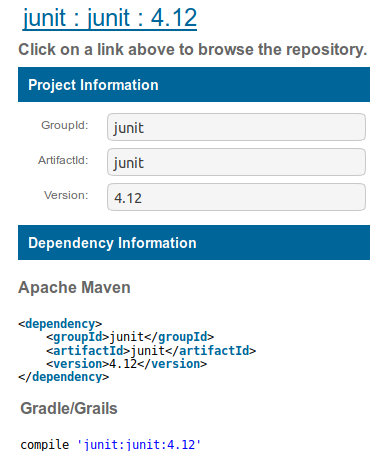
\includegraphics[width=0.4\linewidth]{HowToUse/3DependencyManagement/javaDep/gradleInMavenRepo.png}
\end{figure} 
Possiamo notare ora la differenza sostanziale della configurazione delle dipendenze tra il pom.xml di Maven e la build.gradle di Gradle. A questo punto per scaricare le dipendenze si deve eseguire il comando \texttt{dependencies} il cui output restituirà una lista di tutti i task con le relative dipendenze associate.

\end{flushleft}
\end{document}
